\section{Drivers of Regional Differences in Wind Value}\label{sec:regional_drivers}

The previous section established that the market value of wind energy declines with penetration and that this decline propagates across interconnected markets. Yet the rate and severity of this decline are far from uniform across Europe. A wind farm in Sweden earns a fundamentally different return per megawatt-hour than one in Germany, even when both face similar wholesale price levels, because the underlying market structures, flexibility resources, and wind generation patterns differ profoundly. This section examines three principal drivers of regional variation: the physical wind resource and its spatial characteristics, the architecture and composition of electricity markets, and the level of existing wind penetration, which determines where each market sits on the cannibalisation curve.

\subsection{Wind Resources and Spatial Patterns}\label{sec:wind_resources}

\subsubsection{Atmospheric Circulation and Regional Wind Climates}\label{sec:wind_climates}

European wind energy is governed by the large-scale westerly circulation that carries Atlantic weather systems eastward across the continent. Recurrent weather regimes modulate this flow. Grams et al. \cite{Grams2017} identified seven such regimes through clustering of sea-level pressure fields: three cyclonic regimes that collectively drive strong westerly flow on 38.2\% of winter days, and four blocked regimes (38.8\%) that stall high-pressure systems over Scandinavia or Central Europe. European mean wind generation swings from 22~GW during blocking to 44~GW during the Atlantic Trough, a volatility band of 66\% of the winter mean \cite{Grams2017}. The North Sea and Baltic respond in near-lockstep to these large-scale patterns, but their response is not identical: the Baltic's partial shielding by the Scandinavian land mass creates a degree of decorrelation that is relevant for portfolio diversification between the two basins.

\vspace{4pt}

Karagali et al. \cite{Karagali2013}, using satellite-derived wind speed measurements from the pre-2013 period, characterised mean wind speeds of approximately 9.75~m\,s$^{-1}$ over the North Sea compared with 7.5 to 8.0~m\,s$^{-1}$ over the Baltic. The North Sea benefits from direct exposure to the Atlantic fetch, with dominant south-westerly to westerly winds during winter; the Baltic sits in a transitional zone between maritime and continental influences, with more varied wind directions and greater seasonal amplitude \cite{Karagali2013}. These satellite-derived estimates predate the rapid expansion of North Sea offshore capacity and do not capture the cluster wake effects that now reduce effective wind speeds in densely developed areas such as the German Bight, a limitation that complicates direct comparison with the sparser Baltic.

\subsubsection{Capacity Factors: North Sea versus Baltic}\label{sec:capacity_factors}

The difference in mean wind speeds translates directly into a difference in energy yield. Solbrekke and Sorteberg \cite{Solbrekke2022} developed NORA3-WP, a high-resolution (3~km) offshore wind power dataset covering the North Sea, Baltic Sea, Norwegian Sea, and Barents Sea for the period 1996 to 2019. Their results confirm a clear gradient: capacity factors of 40 to 50\% across the central and northern North Sea, 35 to 40\% in the Baltic, and 45 to 55\% along the exposed Norwegian coastline \cite{Solbrekke2022}.

\vspace{4pt}

These figures, however, do not account for inter-farm wake losses, an effect of growing importance as North Sea wind farms proliferate and one that the NORA3-WP dataset, ending before the post-2020 capacity surge, cannot capture. Schneemann et al. \cite{Schneemann2022} analysed wake properties in the German Bight using large-eddy simulations. They found wind speed deficits of 2 to 2.5~m\,s$^{-1}$ within farm clusters that can extend up to 70~km downstream under stable atmospheric conditions. Given the cubic relationship between wind speed and power ($P \propto v^3$), a 10\% speed deficit translates to roughly a 27\% reduction in power output. The German Bight, where multiple gigawatt-scale clusters now operate in close proximity, is particularly affected. The Baltic Sea, with sparser development and greater inter-farm spacing, is less susceptible to cluster wake effects. The gap in effective capacity factors between the two basins may therefore be narrower than raw wind speed data suggest.

\subsubsection{Spatial and Temporal Correlation}\label{sec:correlation}

The correlation structure of wind generation across space and time is a critical determinant of portfolio-level cannibalisation. When wind farms across a region produce simultaneously, they collectively depress the same set of market prices; when their output is decorrelated, the price impact is distributed across different hours, reducing the severity of cannibalisation for each individual asset. Whether the North Sea and Baltic Sea are sufficiently decorrelated that spreading investment across both basins reduces overall cannibalisation exposure is an open empirical question.

\vspace{4pt}

Wind power correlation decays exponentially with distance, a pattern documented from transcontinental \cite{Louie2014} to European scales \cite{Olauson2016}, but the decay is neither isotropic nor uniform across settings. Directionally, east--west wind farm pairs exhibit a systematic time lag reflecting the west-to-east propagation of Atlantic fronts, so that a wind event in the North Sea precedes the corresponding Baltic event by several hours \cite{Malvaldi2017}. This directional dependence partially decorrelates the two basins even under the same synoptic pattern, and cross-basin correlations are consistently lower than within-basin correlations \cite{Olauson2016}. Importantly, correlation decay is slower offshore than onshore: Potisomporn et al. \cite{Potisomporn2022} found this in UK waters, implying that the effective decorrelation length in offshore settings may exceed land-based estimates.

\vspace{4pt}

\begin{figure}[ht]
    \centering
    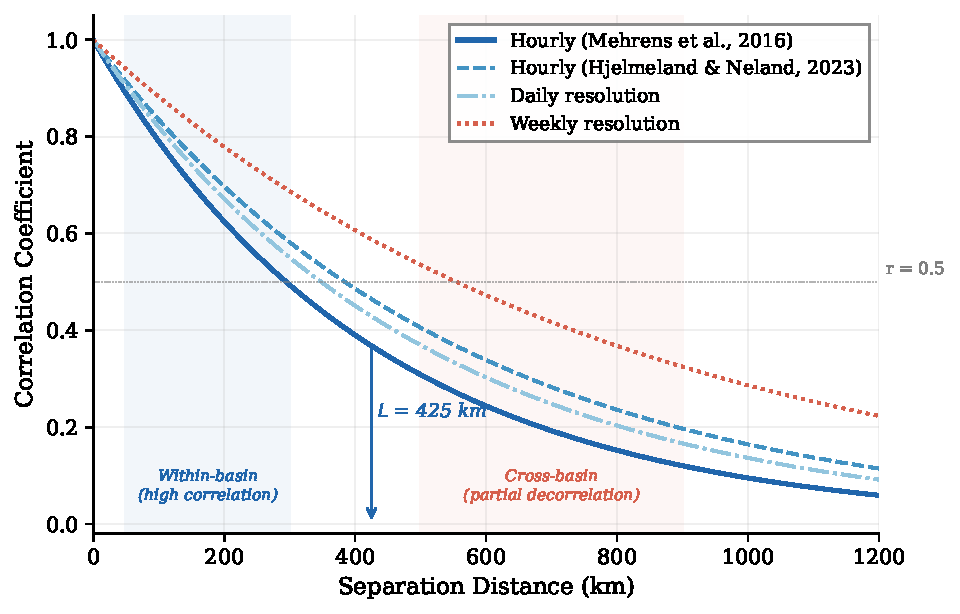
\includegraphics[width=0.75\textwidth]{correlation_decay.pdf}
    \caption{Exponential decay of wind power correlation with separation distance at different temporal resolutions, based on Mehrens et al. \cite{Mehrens2016} and Hjelmeland and Neland \cite{Hjelmeland2023}. Typical within-basin distances (50--300~km) exhibit high correlation, while cross-basin separations (500--900~km) show partial decorrelation. The decorrelation length $L \approx 425$~km marks the distance at which correlation falls to $1/e$.}
    \label{fig:correlation_decay}
\end{figure}

Mehrens et al. \cite{Mehrens2016} directly quantified the cross-basin correlation structure, finding a decorrelation length of approximately 425~km over the range 4 to 600~km (Figure~\ref{fig:correlation_decay}). Given the North Sea's span of approximately 580~km in width and 960~km in length, and the Baltic's comparable lateral dimensions, this decorrelation length implies that individual wind farms within each basin are strongly correlated at hourly timescales; the German Bight, Dogger Bank, and the Danish North Sea all respond to the same Atlantic weather systems, meaning that high-generation events tend to be basin-wide. If the offshore decorrelation length exceeds the 425~km land-based estimate, as Potisomporn et al. \cite{Potisomporn2022} suggest, within-basin correlation among offshore farms may be stronger still.

\vspace{4pt}

Importantly, the rate of correlation decay depends on temporal resolution. Hjelmeland and Neland \cite{Hjelmeland2023} showed that at hourly resolution the correlation coefficient decays to 0.5 at approximately 384~km, but at weekly and monthly aggregations correlations persist over much larger distances because weather systems span thousands of kilometres. Hourly correlations govern the severity of price depression during individual wind events, while longer-timescale correlations determine whether wind droughts affect both basins simultaneously.

\vspace{4pt}

Critically, while the spatial correlation of wind \textit{generation} has been well characterised, the spatial correlation of electricity \textit{prices} across these basins has not been systematically mapped in relation to wind output. The distinction matters: the SDAC market coupling mechanism transmits price effects across borders, so prices in physically distant but well-interconnected zones can be more correlated than their wind resources. Whether the partial decorrelation of wind output between the two basins translates into a corresponding decorrelation of capture prices, or whether market coupling erodes this diversification benefit, is an open empirical question with direct consequences for cross-basin investment allocation.

\vspace{4pt}

In synthesis, the North Sea offers a stronger wind resource but faces a critical constraint: its high spatial correlation concentrates wind-driven price depression into the same market hours basin-wide, compounding the cannibalisation effect. The Baltic offers a weaker resource, but partial decorrelation from the North Sea and sparser development create a temporal distribution of wind events, so high-generation hours are less perfectly synchronised. Whether this physical trade-off translates into an economic advantage depends entirely on the market structures into which each basin sells, examined in the following subsection.

\subsection{Market Structure and Price Formation}\label{sec:market_structure}

\subsubsection{European Electricity Market Architecture}\label{sec:market_architecture}

The revenue that wind generators earn depends not only on the physical resource but on the design of the market in which they sell their output. The day-ahead market, typically accounting for 80 to 90\% of merchant wind revenue \cite{Jansen2020}, clears through the Single Day-Ahead Coupling (SDAC) mechanism, which employs the EUPHEMIA algorithm to simultaneously match orders across all participating European bidding zones \cite{EUPHEMIA2020}. Germany exemplifies this architecture in practice: when North Sea wind farms submit zero-bid offers into the German-Luxembourg (DE-LU) bidding zone, the SDAC algorithm simultaneously calculates the price impact in DE-LU, checks interconnection capacity to neighbouring zones (Netherlands, Denmark, France), and adjusts all zonal prices to reflect the marginal value of transmission. The price in any given zone reflects both domestic supply-demand conditions and the marginal value of interconnection with neighbours \cite{EUPHEMIA2020, Newbery2018}. This coupling is what transmits the merit order effect across borders, making the North Sea and Baltic markets interdependent in a way that national-level analyses cannot capture. For this thesis, the implication is direct: any model of wind capture value must treat both basins as a single coupled system rather than two independent markets.

\subsubsection{Bidding Zones Around Each Basin}\label{sec:bidding_zones}

The geographic resolution at which prices are formed directly affects wind capture values. European electricity markets are divided into bidding zones, each clearing at a single price; Figure~\ref{fig:bidding_zones} provides a schematic overview across both basins. North Sea offshore wind sells into a set of large, relatively liquid bidding zones: Germany-Luxembourg (DE-LU), the Netherlands (NL), Belgium (BE), Denmark-West (DK1), and the five Norwegian zones (NO1 to NO5), along with the United Kingdom. Germany's single bidding zone, which masks significant north-south congestion, remains under review \cite{Egerer2015, GermanBZSplit2024}; a potential split would directly affect North Sea wind capture values by creating a low-price northern zone.

\vspace{4pt}

The Baltic basin is served by a more fragmented set of bidding zones that reflects both the Nordic tradition of zonal pricing and the legacy of post-Soviet electricity systems. The Nordic countries pioneered multi-zone market design: Sweden is divided into four zones (SE1 to SE4), Norway into five (NO1 to NO5), and Denmark into two (DK1 and DK2). Fridolfsson and Tanger\aa{}s \cite{Fridolfsson2009} found that this multi-zone structure operates without systematic market power abuse, with transmission constraints creating natural price areas that reflect genuine physical congestion. Finland operates as a single zone, and Poland clears as one zone despite significant internal congestion. The three Baltic states (Lithuania, Latvia, and Estonia) each constitute their own bidding zone \cite{ACER2025}. In February 2025, the three Baltic states completed synchronisation with the continental European grid, disconnecting from the Russian and Belarusian power system \cite{BalticSynchronisation2025}, this reshaped cross-border flow patterns and exposed Baltic prices more directly to Nordic and Central European market conditions \cite{ACER2025}.

\begin{figure}[ht]
    \centering
    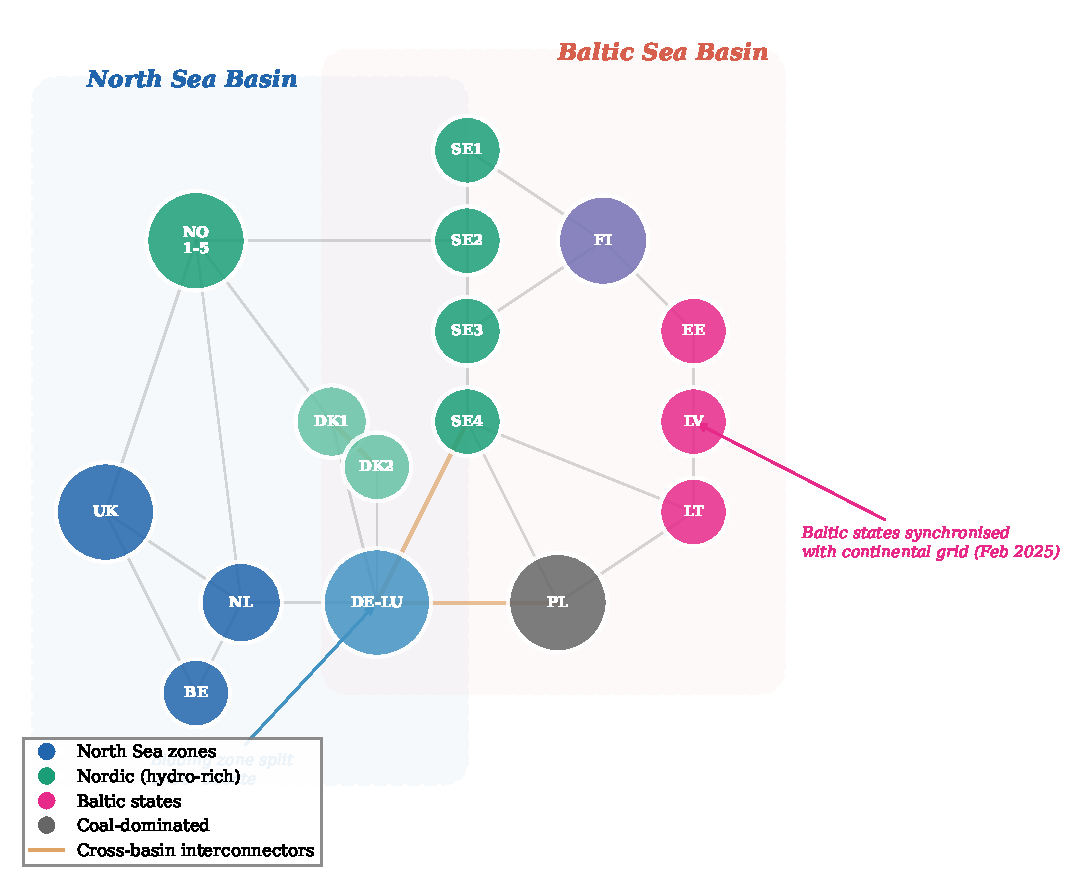
\includegraphics[width=0.75\textwidth]{bidding_zones_map.pdf}
    \caption{Schematic map of bidding zones and key interconnectors around the North Sea and Baltic Sea basins. Node colours indicate market archetype: blue for North Sea zones, green for hydro-rich Nordic zones, pink for Baltic states (synchronised with the continental grid in February 2025), and grey for coal-dominated systems. Orange lines highlight cross-basin interconnectors.}
    \label{fig:bidding_zones}
\end{figure}

Cross-border transmission capacity determines the extent to which price differences can be arbitraged away. Flow-based capacity calculation in the Nordic region and the EU Clean Energy Package's requirement that member states make at least 70\% of cross-zonal capacity available for trade are both pushing markets toward greater price convergence \cite{ACER2023, ACER2025}. The ENTSO-E Offshore Network Development Plan envisions more than \euro{}400~billion of offshore transmission investment by 2050 to support 189~GW of combined North Sea and Baltic capacity \cite{ONDP2024}. For wind generators, greater convergence is double-edged: surplus generation exports more easily, supporting capture values in the exporting zone, but importing zones absorb the corresponding price depression. The contrast in zonal architecture between the two basins matters for capture value analysis: the Baltic's fragmented pricing structure localises price signals, meaning that cannibalisation in one zone does not automatically propagate to neighbours unless interconnection is sufficient.

\subsubsection{Generation Mix and System Flexibility}\label{sec:gen_mix}

The composition of a country's generation fleet determines the shape of its merit order curve, which in turn governs how sensitively wholesale prices respond to changes in wind output. Figure~\ref{fig:gen_mix} compares the generation mix across the key countries bordering each basin. Four archetypes illustrate the range of market environments that offshore wind encounters across the two basins: a large thermal system (Germany), a small but exceptionally interconnected system (Denmark), a hydro-dominated system (Sweden), and a coal-heavy emerging market (Poland).

\begin{figure}[ht]
    \centering
    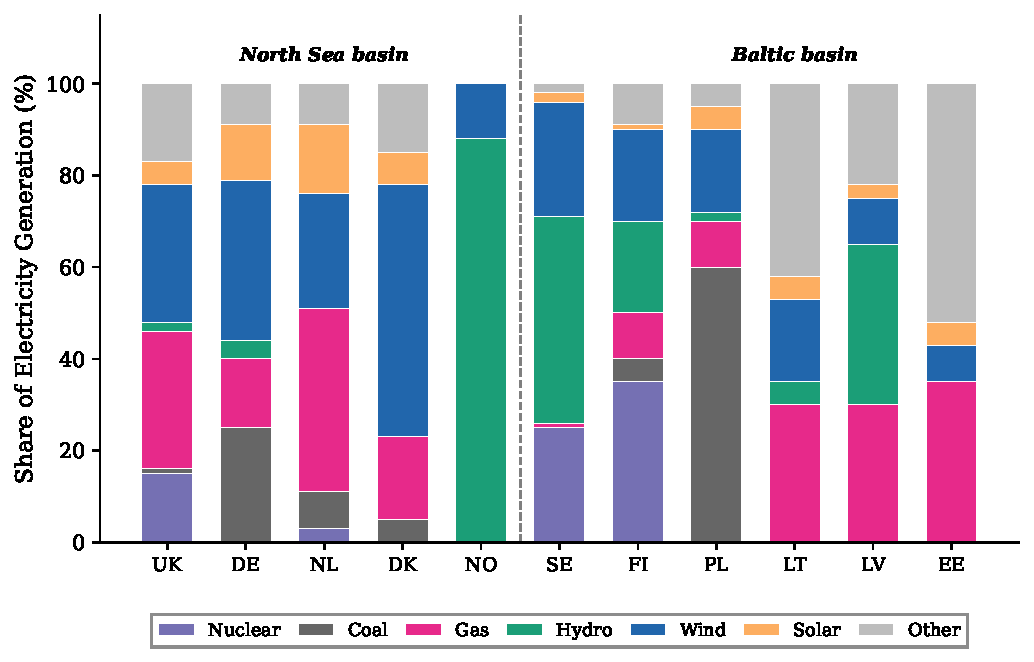
\includegraphics[width=0.9\textwidth]{generation_mix_comparison.pdf}
    \caption{Electricity generation mix across North Sea and Baltic basin countries (approximate 2024 shares). Thermal-heavy systems (Germany, Poland) exhibit steep merit order curves where wind output produces large price swings; hydro-dominated systems (Sweden, Norway) absorb variability with minimal price impact. This diversity in generation portfolios is the primary structural driver of cross-basin differences in wind capture value. Data from Ember \cite{Ember2025} and national transmission system operators.}
    \label{fig:gen_mix}
\end{figure}

Germany exemplifies the challenge facing thermal-heavy systems. With a dispatchable generation fleet still dominated by coal, lignite, and gas \cite{Ember2025, EmberGlobal2024}, the German merit order is relatively steep, meaning that each additional unit of wind displacing a marginal gas plant produces a large price swing. When wind generation is high and pushes the clearing price down to the level of lignite must-run capacity or inflexible combined heat and power plants, the price drop is severe. Combined with Germany's position as the largest European electricity market, this volatility propagates through SDAC to the Netherlands, Denmark, and beyond \cite{GermanPrices2023}.

Denmark presents a contrasting case. Despite the highest wind penetration in Europe, approximately 55\% of electricity generation \cite{DanishEnergyAgency2024, Ember2025}, Danish wind value factors have not collapsed as rapidly as theory would predict, because Denmark is exceptionally well interconnected relative to its size. Western Denmark has direct interconnections to Norway and Sweden, both of which offer large-scale hydropower storage that absorbs surplus Danish wind during windy periods and exports back during calm spells. This hydraulic flexibility effectively flattens the merit order curve that Danish wind generators face \cite{Hirth2013}.

Sweden's hydro-dominated generation mix, approximately 45\% of electricity production \cite{Ember2025}, provides the most favourable market environment for wind energy in the Baltic region. Hydropower reservoirs in northern Sweden act as a natural battery, storing potential energy during high wind and releasing it when wind falls. Hirth \cite{Hirth2013} estimated that at 30\% wind penetration, the wind value factor is approximately 18\% higher in hydro-dominated systems than in thermal-dominated systems, which is a gap large enough to shift a marginal project from loss-making to viable, and one that structurally favours Baltic offshore wind selling into Swedish zones over North Sea wind selling into German ones.

\vspace{4pt}

At the opposite end of the spectrum, Poland occupies a unique position on the Baltic rim. Its generation mix remains dominated by coal, still exceeding 60\% in 2024 \cite{EmberGlobal2024}, with only nascent offshore wind development. Because wind energy displaces some of the most carbon-intensive and expensive generation in the European merit order, new offshore wind in Poland earns high capture values in the near term. Poland has planned 5.9~GW of Baltic offshore wind by 2030, a programme that would constitute the largest single addition of zero-marginal-cost capacity the Polish system has experienced \cite{Owczarek2021}. As this capacity enters the market, it will progressively displace the coal-fired units that currently set marginal prices during high-demand hours, flattening the merit order and eroding the very conditions that make early projects attractive. Whether favourable capture values persist therefore depends on the pace at which coal retires relative to the pace at which offshore wind is added.

\vspace{4pt}

The contrast is sharp: an offshore wind farm in Sweden's SE4 zone and one in the Polish Baltic, separated by a few hundred kilometres, inhabit fundamentally different economic realities, with the former hydro-buffered and resilient to price depression, and the latter earning high capture prices today from displacing expensive coal but facing steep cannibalisation as 5.9~GW of new capacity enters a market with limited flexibility. Two further Baltic markets are entering the development cycle: Finland enacted its offshore wind act in January 2025 \cite{FinlandOffshoreWind2025}, enabling 6.5~GW by the late 2030s in a nuclear- and hydro-dominated system, while Estonia secured EU approval for a \euro{}2.6~billion support scheme in December 2024 \cite{EstoniaOffshoreWind2025}. Both sit at the very beginning of the penetration curve, offering near-zero cannibalisation today but facing rapid transitions as planned capacity materialises.

\vspace{4pt}

Table~\ref{tab:country_archetypes} consolidates the key characteristics of each market archetype discussed above. The cross-basin comparison becomes visible at once: the wind value factors that emerge are starkly different.

\begin{table}[ht]
\centering
\small
\caption{Summary of market archetypes across the North Sea and Baltic Sea basins. Wind penetration and value factor estimates reflect approximate 2024 values. The final column indicates the dominant revenue support instrument for offshore wind.}
\label{tab:country_archetypes}
\resizebox{\textwidth}{!}{%
\begin{tabular}{l c c l l c c l}
\toprule
\textbf{Country} & \textbf{Basin} & \textbf{Wind (\%)} & \textbf{Dominant gen.} & \textbf{Flexibility} & \textbf{Intercon.} & \textbf{Value factor} & \textbf{Support} \\
\midrule
Germany & NS & $\sim$35 & Gas, coal, wind & Limited; gas peakers & Medium & 0.76--0.85 & Two-sided CfD \\
\addlinespace
Denmark & NS/BS & $\sim$55 & Wind, gas & Nordic hydro (import) & Very high & 0.80--0.90 & CfD (from 2025) \\
\addlinespace
Netherlands & NS & $\sim$25 & Gas, wind & Gas peakers; import & High & 0.85--0.90 & SDE++ tender \\
\addlinespace
UK & NS & $\sim$30 & Gas, wind, nuclear & Gas CCGT; storage & Medium & 0.80--0.85 & CfD (AR rounds) \\
\addlinespace
Sweden & BS & $\sim$25 & Hydro, nuclear, wind & Large hydro reservoirs & High & 0.90--0.95 & Elcert. (phasing out) \\
\addlinespace
Finland & BS & $\sim$20 & Nuclear, hydro, wind & Hydro; nuclear baseload & High & 0.90--0.95 & Premium / CfD \\
\addlinespace
Poland & BS & $\sim$18 & Coal, gas & Limited; coal inflexible & Low & 0.95--1.00 & CfD auction \\
\addlinespace
Baltic states & BS & $<$15 & Gas, import, wind & Limited; import-dep. & Medium & $\sim$1.00 & Premium schemes \\
\bottomrule
\end{tabular}%
}
\end{table}

The pattern the table reveals is striking: every Baltic market records a higher value factor than every North Sea market, despite uniformly lower interconnection and, in Poland's case, near-zero system flexibility. Penetration level, not flexibility access, appears to be the dominant predictor of current value factor levels. Whether this ordering persists as Baltic capacity scales from single-digit to double-digit gigawatts is the question that a cross-basin comparison must answer.

\subsubsection{Price Levels and Convergence Across Basins}\label{sec:price_comparison}

For wind generators, absolute price levels matter less than the relationship between wind output and prices. German wholesale prices averaged above 50~\euro/MWh through 2022 and 2023, while Nordic zones traded at significantly lower levels \cite{GermanPrices2023, ACER2025}. But a high average wholesale price is of limited value if capture prices fall substantially below it. The critical distinction between the two basins is their sensitivity to wind generation: the same wind event produces a deeper price depression in the German Bight than in the Swedish Baltic, even when the volume of generation is comparable. These price sensitivities have not been systematically mapped across the full set of bidding zones surrounding both basins.

\vspace{4pt}

Market structure and generation mix create a fundamental bifurcation in how the two basins absorb wind variability. Hydro-rich Nordic systems (Sweden, Norway, Finland) possess the flexibility to absorb concentrated wind output with minimal price impact: during high wind hours, water is stored instead of spilled, and during calm periods stored energy is released, flattening the merit order curve. Thermal-heavy systems (Germany, Poland) lack this buffer: when wind is high, inflexible coal and nuclear generation must be kept online or ramped down at cost, creating an abrupt price collapse that depresses capture values for all generators, not just wind. This structural difference means that two wind farms with identical generation profiles would earn fundamentally different revenues depending on which market they sell into. North Sea wind entering thermally-dominated zones (Germany, Benelux) experiences steep capture value degradation; Baltic wind selling into hydro-rich zones retains value. The question for cross-basin investment is whether superior North Sea wind resources compensate for less favourable market absorption, or whether market structure advantages in the Baltic outweigh lower physical resource quality.

\subsection{The Penetration Gradient}\label{sec:penetration_gradient}

A third factor mediates the interaction between wind resources and market structure: the existing level of wind penetration. Where a market sits on the cannibalisation curve determines the marginal impact of each additional gigawatt.

\vspace{4pt}

North Sea markets are already mature wind markets. Denmark generates approximately 55\% of its electricity from wind \cite{DanishEnergyAgency2024}, Germany approximately 35\%, the Netherlands approximately 25\%, and the United Kingdom approximately 30\% \cite{Ember2025, WindEurope2024Stats}. These markets have experienced significant value factor erosion over the past decade. Baltic markets, with the partial exception of Sweden (approximately 25\% and heavily buffered by hydro), are earlier on the penetration curve: Finland at approximately 20\%, Poland at approximately 18\%, and the Baltic states below 15\% \cite{Ember2025, EmberGlobal2024}.

\vspace{4pt}

Both basins have committed to dramatic expansion, underpinned by the broader EU targets set out in REPowerEU \cite{REPowerEU2022}. The Esbjerg Declaration of May 2022 pledged at least 65~GW of combined North Sea offshore wind by 2030 and 150~GW by 2050 \cite{Esbjerg2022}. Three months later, the Marienborg Declaration committed eight Baltic rim countries to at least 19.6~GW of Baltic offshore wind by 2030, a sevenfold increase from the 2.8~GW installed at the time \cite{Marienborg2022}. Barzehkar et al. \cite{Barzehkar2024} estimate 93~GW of technical potential in the Baltic basin through GIS-integrated LCOE modelling, suggesting that the Marienborg target represents only a fraction of what is physically and economically viable. The ENTSO-E Offshore Network Development Plan consolidates these ambitions into a system-wide projection of 146~GW in the North Sea and 43~GW in the Baltic by 2050 \cite{ONDP2024}.

\vspace{4pt}

As both basins expand simultaneously, cannibalisation will intensify across all markets, but the timing and severity will differ. North Sea markets, already at high penetration, face the steepest marginal declines in capture value. Baltic markets are earlier on the curve and, in the case of Poland and the Baltic states, stand to benefit from displacing expensive thermal generation. The question that this divergence raises is fundamentally a spatial and temporal forecasting problem: given the planned trajectories of expansion in each basin, what will capture values look like in 2030 and beyond? Answering this requires the modelling tools examined in the following section.

\subsection{Section Summary}\label{sec:regional_summary}

Three factors interact to create fundamentally different wind value environments around the North Sea and Baltic Sea: the wind resource (stronger but more spatially correlated in the North Sea; weaker but partially decorrelated in the Baltic), the market structure (hydro-dominated Nordic systems absorb variability with minimal price impact; thermal-heavy systems amplify it \cite{Hirth2013, Keppler2016}), and the level of existing penetration (mature North Sea markets already experiencing significant value erosion; Baltic markets in an earlier, more favourable phase). Yet the literature has not systematically compared capture values across these two basins under planned expansion scenarios.
